% !TEX root = ../main.tex

\chapter{Method}
\label{ch:method}

This chapter presents the core contribution of the project, focusing on the binary tree model with a particular emphasis on two key functions. The efficiency of the model was tested on two OpenAI Gym environments, which will be discussed. Additionally, some basic reinforcement learning components and their adaptations for this project will be presented. The code for this chapter is written in Python and can be found on Github\footnote{$https://github.com/DavidGauc/btree\_model/$}.

\section{Model}
Models are tools used to represent a range of functions, and the number of functions a model can represent depends on the specific model used. However, every model can only approximate a finite number of functions.

This project employs binary trees as a unique method to approximate control policies using the reinforcement learning approach. Compared to traditional neural network models, binary trees offer potential benefits, including improved performance and interpretability. Additionally, binary trees do not require back-propagation or continuous functions, which makes them a more efficient and effective solution.

The binary tree model is being used to solve continuous control problems in this project. It takes in information about the current state of the environment and outputs the appropriate action for the agent to take. The goal is to use the binary tree to approximate the best action for the agent to take given the current state, making the model an effective tool to approximate control policies.

\subsection{\texttt{Node} module}
A node in a binary tree is composed of a pointer that points to its parent node, a function from a defined function class, and an assigned weight that adjusts the importance of the decision or computation made at that node. Additionally, the node has two pointers - one to its left child and one to its right child - that are used to traverse the tree and make decisions based on the input data and the functions applied at each node. The basic functioning of this module was already implemented at the beginning of the project. An important addition that needs to be made is to have a pointer to the parent, which was not necessary before having a method to dynamically increase the tree size. Each node in the tree needs to know its parent node in order to transmit the updated number of weights and nodes once new nodes are added to the tree, as you will see in \ref{model_functioning}. Figure~\ref{fig:node_composition} illustrates a binary tree with a single node to show the different elements that compose a node in this model and the pointers that are assigned to it.
\begin{figure}[!ht]
\centering
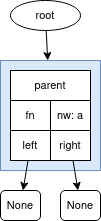
\includegraphics[width=.2\textwidth]{node}

\caption[Components of a single-node tree]{
  \textbf{Components of a single-node tree}
Representation of a binary tree with a single node. The $root$ pointer points to the node, and the $parent$ pointer points to nothing as it is a single-node tree. The main components of the node are a function $fn$ that is implemented in the function module, an amount of weights $nw$ it contains, and two pointers to its left and right child ($left$, $right$) which point to None in this case.
 }
\label{fig:node_composition}
\end{figure}

\subsection{\texttt{Functions} module}
Each node in the binary tree contains a function that is used to make decisions or perform computations based on the input data. In the project, three function types were implemented: constant, linear, and perceptron.

The constant function returns the weights as output regardless of the input values, while the linear function returns the dot product of the weights and the observations it received as input. The perceptron uses the sigmoid activation function
\begin{equation}
\frac{1} {(1 + \exp(-x))}
\end{equation}
 to transform the dot product between the weights and observations (denoted as $x$) into a scalar value that can be used to perform computations.

Each instance of the function class contains the number of inputs and outputs, the weights used by the function, and the number of times the function has been activated. The weights can be learned or fixed, and the input and output values can take a specific range.

The module also includes a way to set the required amount of weights needed for each function and return the unused weights. Additionally, it increases a counter each time a function is activated in the tree. This allows us to see which nodes and functions were activated the most during the process, which is important for analysis, especially when determining which tree structure is most convenient for solving different problems.

An important add-on that was implemented in this project is the ability to copy a function. This feature will be used in the node insertion strategy presented later.

For non-leaf nodes in the tree, it is convenient to use linear functions because their output will be a scalar value that is useful for traversing the tree. The details of how the functions, weights, and pointers are used to make decisions and perform computations in the tree can be found in the activate function in \ref{binary_tree}.

\subsection{\texttt{BTree} module}

\label{binary_tree}
This module implements the binary tree model. A binary tree is composed of interconnected nodes, each of which holds a function. The illustration in Figure~\ref{fig:tree_composition} shows a binary tree with a root node and two child nodes.
\begin{figure}[!ht]
\centering
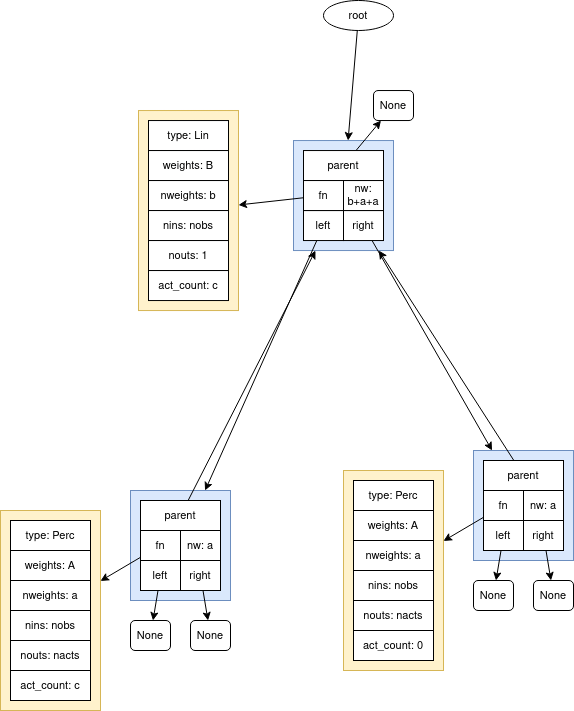
\includegraphics[width=1\textwidth]{tree}
\caption[Components of a tree with three nodes]{
  \textbf{Components of a tree with three nodes}
Representation of a tree with a root node that contains a linear function and two child nodes with perceptrons. Each node displays its pointer to the corresponding function instance (represented by yellow blocks) and the connections to each other. The number of weights $nw$ of the parent node is incremented by the number of weights of its children nodes.
 }
\label{fig:tree_composition}
\end{figure}
A binary tree is a structure made up of linked nodes that contain functions that are used to make decisions or perform computations based on input data. Each node in the tree has a function, which can be one of the types implemented in the project: constant function, linear function, or perceptron. It also has two child nodes that can be either leaf nodes or internal nodes.

The module enables the retrieval of basic information about the binary tree, such as its current structure, the number of weights or nodes it has, and the activations that occurred during an experiment. The main contribution of this project is enabling the tree to grow dynamically with a specific node insertion strategy, which will be presented in \ref{model_functioning}.

\subsection{model functioning}
\label{model_functioning}

The process of using the tree to make decisions or perform computations is referred to as activation. This procedure enables the use of a classical data structure like the binary tree for solving reinforcement learning problems. The model uses the reinforcement learning paradigm by getting observations as inputs and outputting actions for the agent to take through the activation of the binary tree. The resulting activation of the model is a good policy approximator which makes use of the advantages discussed in the introduction. An important role is taken by the function that determines how to traverse the tree in such a way that the observations result in convenient actions for the agent to take by getting information about the current state of the environment. The function implemented for this model is represented as pseudocode in Algorithm~\ref{algo:pseudo_activate_function}. The \texttt{activate\_function} starts at the root of the tree and navigates through the links between nodes based on the output of the current node's function. The functions that are not leaf nodes use a linear function in the case of this project. This means the function takes the observations as inputs and gives out a scalar. If the value of the scalar is positive, the left child node is chosen, else the right child node is chosen. By repeating this, the function will eventually get to the bottom of the tree. When reaching a leaf node, the function will return the output obtained by passing the observations as input to the function implemented in that particular node. In the case of this project, leaf nodes will either use a constant function or perceptrons. The outputs will need to be interpreted differently depending on whether the action space is discrete or continuous, as you will see in \ref{env_model_interface}. But basically, this will tell the agent which actions it should perform.

The construction of the tree involves determining the decision points in the tree, which are selected based on the input data and the problem to be solved. The tree can be trained and updated by adjusting its functions, weights, and links between nodes.

Compared to other models like neural networks and decision trees, binary trees have both advantages and limitations. One advantage is interpretability, as the decision points and functions used in the tree can be explained. However, the efficiency of the tree is sensitive to its size, which can be a limitation. This can be mitigated through pruning techniques or other methods that optimize the tree structure.

\begin{algorithm}
\caption{\texttt{activate} function}
\label{algo:pseudo_activate_function}
\begin{algorithmic}[1]
\Function{activate}{$obs$}
\State $node \gets \texttt{self.root}$\Comment starting from the root 
\While{True}
\If{$node$ is a leaf}
    \Return $node.fn(obs)$ \Comment output of $node$'s function
\ElsIf{$node.fn(obs) >= 0$} 
    \State $node \gets node.left$ \Comment go to the left child node
\Else 
    \State $node \gets node.right$ \Comment go to the right child node
\EndIf
\EndWhile
\EndFunction
\end{algorithmic}
\end{algorithm}

The difficulty of tasks can vary, making it necessary to have the ability to adjust the size of the tree accordingly. For instance, simpler problems like the Cartpole in OpenAI Gym can be solved with a smaller tree, while more complex problems demand a larger tree. Increasing the size of the tree enables more complex decision-making and can enhance the model's performance. However, it also increases the risk of overfitting.

In this project, a function has been implemented to dynamically increase the size of the tree as the complexity of the problem increases. This process of finding an optimal structure is referred to as architecture search. The implemented function demonstrates only one of many possible techniques for growing the tree structure. This technique is a simple approach and will add only a minimal amount of complexity while maintaining the model's invariance. It is important to note that the strategy is restricted in the sense that it can only add nodes and not remove them, the functions of the added nodes are taken from the previous tree, and the nodes are added by randomly selecting the place where they will be added. All of these factors can be changed in order to create new strategies that will further develop architecture search for binary trees.

The initial idea was to add one new node at a time, but it was quickly abandoned because it would not maintain the invariance of the model. For example, imagine an initial tree with five nodes, where the output of the linear function in the root decides to go to the left node and from there on, the linear function of that node decides to go to its right node. If we add one new node as a left child of that particular node, the model of the node would have changed because the relative position of the node before the addition is not maintained. This is a problem in our case where we want to add the minimal amount of new complexity while keeping the model invariant.

Therefore, another solution was to add two new nodes directly as child nodes, but this also presented difficulties in maintaining the same model within the new, larger tree structure. In this case, the node that has the same relative position to its parent as the node had before the insertion to its parent would need to take over the function and properties of the old leaf in order to maintain this invariance. That's when the idea of having one of the newly inserted nodes as the parent of the leaf node where the nodes will be inserted, and the other new node as its sibling emerged. In this way, the leaf node will remain a leaf while keeping the whole model invariant.

Another decision that had to be made was whether to maintain the activations upon growing the tree. Initially, the idea was to reset the activation counter when adding the nodes. However, with the new implementation, it was more accurate to take over the current activations for the node that was set as the new parent and to set the counter to zero for the node put as the sibling. This approach helped maintain the model invariant.

Finally, the number of weights and nodes needed to be updated throughout the tree when inserting the new nodes. This issue surfaced once the tree implementation was completed, and it did not work correctly because the nodes did not get the correct amount of weights for their functions to perform. To resolve this, a pointer for each node of the tree was added to its parent node. This allowed traversing the tree from bottom to top while updating the number of weights and nodes during the traversal.

The actual strategy for randomly selecting the place to add two new nodes proceeds as follows:

\begin{itemize}
\item It begins by traversing the tree randomly until it reaches a leaf node. The pseudo code shown in Algorithm~\ref{algo:pseudo_pickrandom_function} illustrates the implementation of the $pick\_random\_leaf$ function which does this job
\item It verifies if the selected leaf is the root of the tree or not
\item If it is, a new parent node is created
\item If not, the leaf's parent node is duplicated to create a new parent node
\item The new parent node is then set as the parent of the current leaf node and its duplicate.
\end{itemize}

The new nodes are added to the tree in such a way that the current leaf node's relative position to its previous parent node remains unchanged.For more details about the implementation the pseudo code of the function is shown in Algorithm~\ref{algo:pseudo_add_node_function}.

\begin{algorithm}[!ht]
\caption{\texttt{pick\_random\_leaf} function}
\label{algo:pseudo_pickrandom_function}
\begin{algorithmic}
\Function{pick\_random\_leaf}{}
\State $current \gets \texttt{self.root}$ \Comment starting from the root 
\State $last\_direction \gets \texttt{None}$ 
\While{$current$ is not the leaf}
\If{$random >= 0.5$} \Comment $random$ is between 0 and 1
\State $current \gets current.left$ \Comment go to the left child node
\State $last\_direction \gets 'left'$ \Comment store relative position of current node to its parent
\Else 
\State $current \gets current.right$ \Comment go to the right child node
\State $last\_direction \gets 'right'$ 
\EndIf
\EndWhile
\Return ($current, last\_direction$)
\EndFunction
\end{algorithmic}
\end{algorithm}

It is important to note that the function does not add two child nodes directly to the leaf node, but instead adds one node as the parent of the leaf node and the other as its sibling. As shown in Figure~\ref{fig:add_node}, this is an example of adding two nodes to a binary tree. Figure~\ref{fig:add_node_before} shows a binary tree with five nodes before using the node adding strategy. Figure~\ref{fig:add_node_after} then shows the binary tree incremented by two new node with their position in the tree. After the addition of these new nodes, all the links in the tree must be updated, and information regarding the number of weights and the number of descendants must be refreshed. To achieve this, the function employs a process of propagating the information from the current leaf node to the root of the tree.

\begin{figure}[!ht]
    \centering
\begin{subfigure}{.48\textwidth}
    \centering
    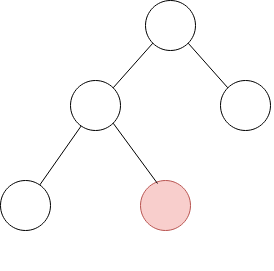
\includegraphics[width=0.6\linewidth]{add_node_before}
    \caption{Illustration of the initial binary tree before the addition of the new nodes. The red node represents the randomly selected leaf node, from which the node addition process will start.} 
    \label{fig:add_node_before}
\end{subfigure}%
\hspace{1em}
\begin{subfigure}{.48\textwidth}
    \centering
    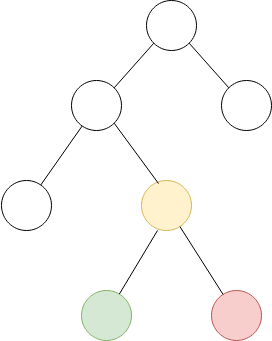
\includegraphics[width=0.6\linewidth]{add_node_after} 
    \caption{Representation of the tree aftesbr adding two nodes using the \texttt{add\_node} function. The yellow node is the newly created parent node and the green node is the sibling of the previously existing red nodesb. It is important to note that the red node retains its relative position to the parent node} 
    \label{fig:add_node_after}
\end{subfigure}
\caption{Addition of two nodes in a binary tree with the \texttt{add\_node} function}
\label{fig:add_node}
\end{figure}


\begin{algorithm}[!ht]
\caption{\texttt{add\_node} function}
\label{algo:pseudo_add_node_function}
\begin{algorithmic}
\Function{add\_node}{}
\State $current, last\_direction = pick\_random\_leaf()$\Comment go to a leaf ($current$) randomly
\If{$current$ is the root}
    \State create $new\_parent$ node with a linear function
    \State take over the number of activations from $current$ to $new\_parent$
    \State $last\_direction \gets 'left'$ \Comment doesn't matter if its the root
    \State $\texttt{self.root} \gets new\_parent$ \Comment $new\_parent$ is the root
\Else
    \State copy $current$'s parent into $new\_parent$ node
    \State take over the number of activations from $current$'s parent to $new\_parent$
\EndIf
\State create $copy\_node$ \Comment copy of $current$
\If{$last\_direction$ is 'right'}\Comment maitain relative position to parent node
    \State $new\_parent.right \gets current$ \Comment set $current$ as right child of $new\_parent$
    \State $new\_parent.left \gets copy\_node$
\ElsIf{$last\_direction$ is 'left'}
    \State $new\_parent.left \gets current$
    \State $new\_parent.right \gets copy\_node$
\Else
    \State raise error
\EndIf

\State Set $new\_parent$'s parent to $current$'s parent\Comment fix parent links
\State Set $current$'s parent to $new\_parent$
\State Set $copy\_node$'s parent to $new\_parent$

\If{$new\_parent$ is not the root}
    \If{$last\_direction$ is 'right'}
        \State set $new\_parent as right child of its parent node$
    \ElsIf{$last\_direction$ is 'left'}
        \State set $new\_parent as left child of its parent node$
    \Else
        \State raise error
    \EndIf
\EndIf

\If{$new\_parent$ is not the root}
    \State $parent\_iter \gets parent of new\_parent$ \Comment starting point for progating up
    \While{True}
        \State number of wheights of $parent\_iter$ is incremented by wheights of newly created nodes
        \State number of nodes of $parent\_iter$ is incremented by nodes of newly created nodes
        \If{$parent\_iter$ is root}
            \State break
        \Else
            \State Set $parent\_iter$ to its parent \Comment Go one node upwards
        \EndIf

    \EndWhile
\EndIf

\State Add to the number of weights of $new\_parent$ the number of weights of its two children nodes
\State Add to the number of nodes of $new\_parent$ the number of nodes of its two children nodes

\EndFunction
\end{algorithmic}
\end{algorithm}

The function for expanding the size of the tree adapts to the complexity of the problem by growing based on a stagnation threshold, which is determined by a lack of improvement in the score for a certain number of steps. A larger tree has a greater search space, which enables it to handle more complex problems. However, it also increases computational time, making it crucial to strike a balance between expanding the tree too rapidly or too slowly.

\section{Environments}

For this project, two environments from the Box2D category of OpenAI Gym were utilized\footnote{https://www.gymlibrary.dev/environments/box2d/}. These environments are more complex than the "Classical Control" problems and offer greater configurability. Box2D is a 2D physics engine designed for games that enables objects to move in a realistic manner, enhancing game interactivity(\cite{noauthor_box2d_nodate}).

\subsection{Lunar Lander}
The Lunar Lander environment simulates a scenario where a rocket must land between two flags on the surface of the Moon. The rocket has three engines that can either be fired at full speed or turned off. This environment is available in both a continuous and a discrete version. In this project, the discrete version was utilized. For the continuous version to work the output needs to be normalized in order to give out values in the range of -1 and 1. The figure shown in Figure~\ref{fig:lunar_lander} depicts the various states that the rocket can be in during the landing process.

\begin{figure}[!ht]
    \centering
    \begin{subfigure}{.32\textwidth}
        \centering
        \fbox{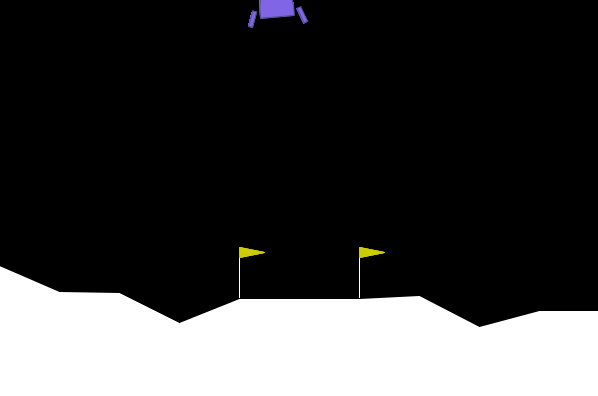
\includegraphics[width=1\linewidth]{start_lunar_lander}}  
        \caption{Illustration of the rocket at the beginning of the task}
    \end{subfigure}
    \hspace{1em}
    \begin{subfigure}{.32\textwidth}
        \centering
        \fbox{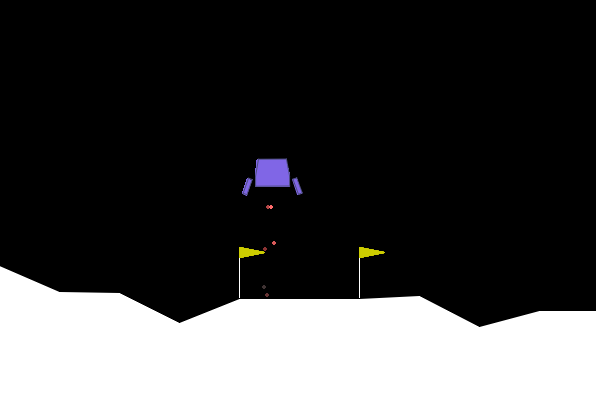
\includegraphics[width=1\linewidth]{fire_lunar_lander}}  
        \caption{Lander firing its main engine in order to adjust its trajectory}
    \end{subfigure}
    \hspace{1em}
    \begin{subfigure}{.32\textwidth}
        \centering
        \fbox{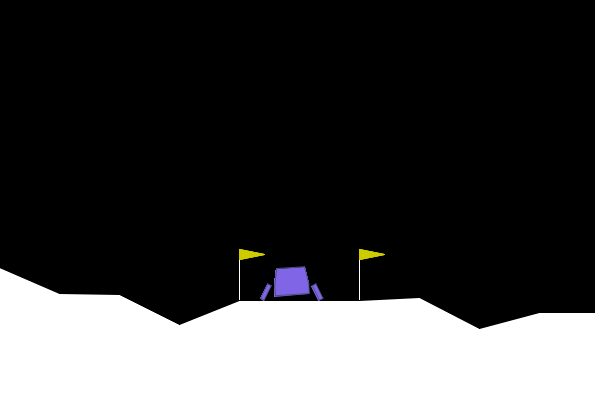
\includegraphics[width=1\linewidth]{land_lunar_lander}}  
        \caption{Successful landing between the two flags}
    \end{subfigure}
    \caption{Different states of the Lunar Lander environmment}
    \label{fig:lunar_lander}
\end{figure}

\subsubsection{Action space}
The environment has four available actions: do nothing, fire the left engine, fire the right engine, or fire the main engine pointing downwards. The strength at which the engines fire cannot be adjusted and is fixed, resulting in a discrete action space with a dimension of 4. In practice the action with the biggest value obtained through the model is chosen and a number from 0 to 3 is sent to the environment.

\subsubsection{Observation space}
The observation space for the Lunar Lander contains eight values.
Two of them are booleans that indicate whether the corresponding leg of the lander is touching the Moon's surface or not, while all the other values are continuous.

\begin{table}[!ht]
\centering
\caption{Observation values for the Lunar lander}
\begin{tabular}[t]{lcc}
\toprule
& Min & Max \\
\midrule
coordinates of the lander in x & -1.5  & 1.5  \\
coordinates of the lander in y & -1.5  & 1.5  \\
linear velocity in x           & -5.0  & 5.0  \\
linear velocity in y           & -5.0  & 5.0  \\
angle                          & -3.14 & 3.14 \\
angular velocity               & -5.0  & 5.0  \\
left leg touching ground       & 0     & 1    \\
right leg touching ground      & 0     & 1    \\
\bottomrule
\end{tabular}
\end{table}%

\subsubsection{Rewards}
For the agent in the Lunar Lander environment, it receives a reward for successfully landing on the landing pad starting from the top of the screen. The reward points in the default implementation are calculated as follow:
\begin{itemize}
  \item $-100 \times \sqrt{state[0] \times state[0] + state[1] \times state[1]}$: This calculates a penalty for the horizontal position and velocity of the lander, where $state[0]$ and $state[1]$ are the normalized horizontal position and velocity, respectively. The closer the lander is to the center of the viewport, the closer the value of $state[0]$ will be to 0, and the less penalty it will incur. The penalty is scaled by -100 to make it a significant factor in the reward.

  \item $-100 \times\sqrt{state[2] \times state[2] + state[3] \times state[3]}$: This calculates a penalty for the vertical position and velocity of the lander, where $state[2]$ and $state[3]$ are the normalized vertical position and velocity, respectively. The calculation is similar to the one for the horizontal position.

  \item $-100 \times \lvert state[4] \rvert$: This calculates a penalty for the angle of the lander, where $state[4]$ is the angle of the lander with respect to the vertical axis. The more the lander is tilted, the higher the penalty.

  \item $10 \times state[6]$: This adds a bonus for having the first leg of the lander in contact with the ground, where $state[6]$ is equal to 1 if the first leg is in contact, and 0 otherwise. The bonus is scaled by 10 to make it a relatively small factor in the reward.

  \item $10 \times state[7]$:  This adds a bonus for having the second leg in contact with the ground. The calculation is similar to the one for the first leg.

  \item $-0.30 \times main\_engine$: This calculates a penalty for each frame the main engine is firing. In the case of a discrete action space $main\_engine$ is either 1 or 0.

  \item $-0.03 \times side\_engine$: This calculates a penalty for each frame the a side engine is firing. In the case of a discrete action space $side\_engine$ is either 1 or 0.

\end{itemize}
An additional reward of -100 or +100 points for crashing or landing safely respectively is obtained at the end of the episode. The final reward is the sum of all of these terms. The design of the reward encourages the agent to land the lander safely on the landing pad with minimum velocity, at a suitable angle, and with both legs in contact with the ground.

The task is considered solved when the agent accumulates a total reward of 200 points or higher. It's worth noting that the exact rewards given for each action, state or event are not fixed and can be adjusted to fine-tune the agent's behavior, based on the specific implementation of the environment.

\subsection{Bipedal Walker}
This environment simulates a two-legged robot attempting to walk as far as possible on uneven terrain. There are two versions available: a "normal" version (Figure \ref{bipedal_normal}) and a more challenging "hardcore" version (Figure \ref{bipedal_hardcore}) which includes obstacles. The robot is composed of a hull and two legs, each with two joints, one connecting to the hull and the other allowing the leg to bend. Figure~\ref{fig:bipedal_walker} illustrates the robot in action on both versions.

\begin{figure}[!ht]
    \centering
    \begin{subfigure}{.48\textwidth}
        \centering
        \fbox{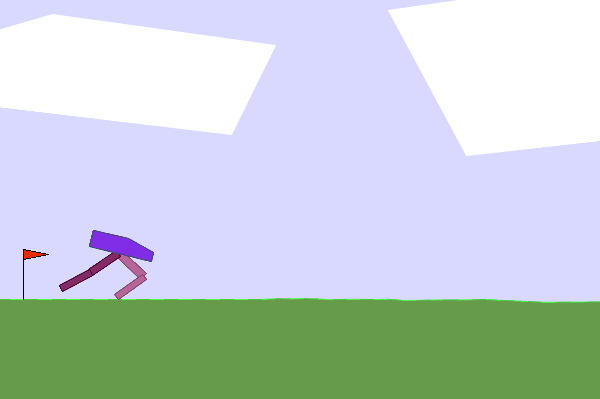
\includegraphics[width=1\linewidth]{bipedal_normal}}
        \caption{Bipedal walker in the "normal" environment version} 
        \label{bipedal_normal}
    \end{subfigure}%
    \hspace{1em}
    \begin{subfigure}{.48\textwidth}
        \centering
        \fbox{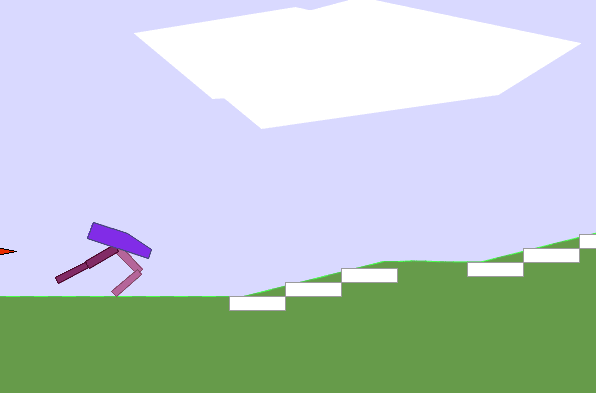
\includegraphics[width=1\linewidth]{bipedal_hardcore}} 
        \caption{Bipedal walker in the "hardcore" environment version} 
        \label{bipedal_hardcore}
    \end{subfigure}
    \caption{Bipedal walker performing on both environment versions}
    \label{fig:bipedal_walker}
\end{figure}

\subsubsection{Action space}
The actions of the bipedal walker are continuous, with four actions available, corresponding to the motor speed values of each joint. The values range from -1 to 1 and determine the movement and stability of the robot. It's possible to adjust the range of values in different implementations of the environment.

\subsubsection{Observation space}
The observation space for the bipedal walker has a dimension of 24 and consists of continuous values, as well as a few boolean values that indicate whether the legs are in contact with the ground or not. The observation space includes information such as the angle, angular velocity, linear velocity, and position of the torso of the robot. It's worth noting that the exact position of the robot is not explicitly stated in the observation space, but it can be derived from other observations, such as the linear and angular velocities of the joints.

\begin{table}[!ht]
\centering
\caption{Observation values for the Bipedal Walker}
\begin{tabular}{lcc}
\toprule
& Min & Max \\
\midrule
hull angle speed                    & -3.14 & 3.14 \\
angular velocity                    & -5.0  & 5.0  \\
horizontal speed                    & -5.0  & 5.0  \\
vertical speed                      & -5.0  & 5.0  \\
position of joints                  & -3.14 & 3.14 \\
joints angular speed                & -5.0  & 5.0  \\
left leg contact with ground        & 0     & 1    \\
right leg contact with ground       & 0     & 1    \\
10 lidar rangefinder measurements   & -1.0  & 1.0  \\
\bottomrule

\end{tabular}
\end{table}%

\subsubsection{Rewards}
A reward is given to the robot when it is able to move forward without falling. Falling is defined as the hull touching the ground (horizontal position less than 0) and it is penalized by -100 points. If the bipedal walker reaches the end of the environment, it accumulates 300 points. The episode is also terminated if the horizontal position of the walker is greater than the length of the terrain. The default calculations for the reward are following:

\begin{itemize}
  \item $ 130 \times pos[0] / SCALE$: This encourages the agent to move forward. $pos[0]$ is the normalized horizontal position of the walker and $SCALE$ is a normalization factor that enables to receive 300 points on completion of the task.

  \item $-5.0 \times \lvert state[0] \rvert$: This calculates a penalty for deviating from keeping the head straight. $state[0]$ is the normalized angular velocity of the walker's head. The more the walker's head deviates from being straight, the higher the penalty.

  \item $-0.00035 \times MOTORS\_TORQUE \times np.clip(\lvert a \rvert), 0, 1)$: This calculates a penalty for the use of motor torque by the agent the calculation is done for each motor of the walker. $MOTORS\_TORQUE$ is a constant that represents the maximum torque that a motor can apply. The larger the torque applied by a motor, the larger the penalty. The use of $np.clip$ ensures that the torque used is clipped to the range $[0, 1]$.

\end{itemize}

The "normal" version is considered solved when 300 points are earned within 1600 time steps. For the "hardcore" version, the same amount of points has to be earned within 2000 time steps. The goal is to achieve the highest possible reward while avoiding falling and moving as efficiently as possible. Like for the Lunar Landar, the values can be adjusted to fine-tune the agent's behaviour.

\section{Control Loop and Performance Evaluation}

To evaluate the efficiency of a model in solving tasks in a given environment, a bridge is needed between the model and the environment. This interface extracts actions from the model, which are then performed by the agent and evaluated in relation to its performance in solving the given problem. It is a crucial component in reinforcement learning algorithms, providing the mechanism for feedback and evaluation of the agent's performance, allowing it to learn and optimize its behavior.

The \texttt{fit} function, at the core of this interface, implements the control loop, evaluating the quality of the agent's actions based on the rewards provided by the environment. The action is extracted from the model. A distinction is also made between environments with a discrete action space and those with a continuous action space, as shown in Figure \ref{env_model_interface}. Once the agent performs the action provided by the model, it receives feedback on the execution of its action. This feedback contains information about the new state of the environment, including the agent itself, as well as a reward that determines if the action was suitable for solving the task. If the problem is solved, the loop finishes.

The efficiency of the agent is calculated by summing the rewards received over the course of a single episode, which is the output of the \texttt{fit} function. This score is used to guide the learning process and update the agent's parameters, helping it to continually improve its performance. The pseudo-code in Algorithm \ref{algo:pseudo_fit_function} illustrates the basic elements of the \texttt{fit} function.





\begin{algorithm}
\caption{\texttt{fit} function}
\label{algo:pseudo_fit_function}
\begin{algorithmic}
\Function{fit}{ind}
\State reset the environment and get the observations
\State set the weights of $ind$ in the model
\State $score \gets 0$
\State $ done \gets False$ \Comment False is a boolean
\For{number of step $nsteps$}
    \State $action \gets env\_model\_interface.get\_action($model,obs$)$
    \State get new state of environment after executing $action$ step
    \State increment $score$ with the obtained reward from the $action$ step
    \If{done}
        \State break
    \EndIf
\EndFor
\Return $score$ \Comment in our case $-score$ as we use CMA-ES
\EndFunction
\end{algorithmic}
\end{algorithm}


\section{Adjusting Action Selection for Discrete and Continuous Control Tasks}
\label{env_model_interface}

When we're trying to control things, like robots or machines, we need to make decisions about what actions to take. These actions can be either specific things to do or more continuous movements. Environments with either a discrete or continuous action space, as well as discrete or continuous observation spaces, need to be distinguished.

OpenAI Gym helps us by telling us whether we're dealing with specific actions or continuous movements. If we're dealing with specific actions, we just use the number of actions in the program. If we're dealing with continuous movements, we need to rescale our actions to make sure they fit within the allowed movements. We create a special program for this, called a lambda function. This lambda function should take as input an action that needs to be between zero and one (e.g., logistic function) and rescale that action into the boundaries allowed for the function.

Next, a function is created to extract the action from the environment and readapt the output to be consistent with the type of action space. This function is used by the control loop to retrieve the action from the model that the agent should execute. The function takes the model and the current observation of the environment as inputs. It first obtains the action through activation of the binary tree. If the environment is determined to be continuous by the above procedure, the action is rescaled and returned as the output. This means that all outputs of the binary tree are used and they correspond to the signal to send to each control, which requires regression to approximate an action based on the given outputs. If the environment is discrete, the function selects the action with the highest activation by examining the leaf reached by the activation of the binary tree. The procedure is outlined in pseudocode in Algorithm~\ref{algo:pseudo_get_action_function}.

\begin{algorithm}
\caption{\texttt{get\_action} function}
\label{algo:pseudo_get_action_function}
\begin{algorithmic}
\Function{get\_action}{model, obs}
\State $action \gets model.activate(obs)$\Comment action obtained from model activation
\If{environment type is continuous}
    \State rescale the $action$ within the action boundaries
\ElsIf{environment type is discrete}
    \State pick $action$ with highest activation
\Else
    \State raise Error
\EndIf
\Return $action$
\EndFunction
\end{algorithmic}
\end{algorithm}

\section{Challenges}

\begin{itemize}
  \item The main difficulty was encountered in implementing the \texttt{add\_node} function. The goal is to generate a model that is functionally equivalent to the previous best performing model but still capable of improvement. This is achieved by adjusting more weights. If improvement is not achieved, the \texttt{add\_node} function can be called again until the critical complexity is reached and better scores are obtained. When adding new nodes, it's important to maintain the direction chosen during activation and the number of times each node's function was activated before the node addition. This means that if a node's function chose to go to the left child node during activation, the new larger tree should also go the same way, and the activation should lead to the same leaf but within a larger tree. The code memorizes the last direction chosen when randomly going through the tree, and when adding new nodes, the randomly selected leaf keeps its relative position to its new parent nodes.

  \item Another challenge was ensuring that each node always knew the number of weights it and its descendants had. This information is crucial for the functions within the nodes. When adding new nodes to a tree, the number of weights for all ancestor nodes of the newly added nodes is no longer correct, as they must now include the number of weights of those newly added nodes. The same holds true for the number of nodes, which also needs to be updated. The number of nodes for a given node corresponds to the number of descendants of that node, including itself. In the implementation of the \texttt{add\_node} function, this information was propagated upward through the tree starting from the parent node of the one of the two newly inserted nodes (the one that is set as parent of the leaf which was chosen randomly). The number of weights and nodes of the newly inserted nodes was added to the current node iteratively. Finally, the number of weights and nodes of the new parent node, which was not included in the loop, was also increased by the number of weights of its two children.
\end{itemize}